\chapter{Tümevarımla İspat}
\label{chap:tumevarim}


\par\smallskip{\sffamily\bfseries\color{cAcc}Öğrenme Hedefleri}\nopagebreak

\begin{itemize}\setlength{\itemsep}{2pt}\setlength{\parskip}{0pt}
\item İyi sıralama ilkesi ile matematiksel tümevarım ilkesi arasındaki ilişkiyi açıklayabilme.
\item Zayıf ve güçlü tümevarımla ispat kurabilme.
\item Matematiksel tümevarımın neden tümdengelimsel olduğunu gerekçelendirebilme.
\end{itemize}

\section*{Bölüme Genel Bakış: Sonlu Adımdan Sonsuz Sonuca}

Matematiksel tümevarım, tek bir hamlede sonsuz sayıda önermeyi kanıtlayan olağanüstü bir araçtır; ama gücü kadar adı da yanıltıcıdır. Yöntemin ilk açık kullanımları Levi ben Gerson ve Francesco Maurolico’ya (16. yüzyıl) uzanır; Blaise Pascal 1654’te aritmetik üçgen üzerine çalışırken ilkeyi sistemli biçimde uyguladı. On dokuzuncu yüzyılda Giuseppe Peano, tümevarımı doğal sayıların tanımlayıcı aksiyomlarından biri hâline getirdi: ℕ, tam da üzerinde tümevarımın çalıştığı yapı olarak kurulur.

Bu bölüm tümevarımın taban–geçiş şemasını, zayıf ve güçlü biçimlerini ve — belki en önemlisi — neden tümdengelimsel bir yöntem olduğunu ele alır. Öğretmen adayı için tümevarım, hem bir matematiksel teknik hem de bilgisayar biliminin özyineleme fikriyle doğrudan bağlantılı, disiplinler arası bir köprüdür; bu yüzden yöntemi yalnızca ‘uygulamak’ değil, ‘neden işlediğini’ kavramak hedeflenir.

\section{İlke}

\begin{tcolorbox}[bookbox,colback=cDef]\textbf{\textsf{\textcolor{cAcc}{Tanım.}}}\quad Matematiksel tümevarım ilkesi: P(n) doğal sayılar üzerine bir önerme olsun. Eğer (i) P(1) doğru [taban adımı] ve (ii) her k için P(k) ⇒ P(k+1) [tümevarım adımı] ise, o hâlde her n ≥ 1 için P(n) doğrudur.\end{tcolorbox}

\begin{figure}[htbp]
\centering
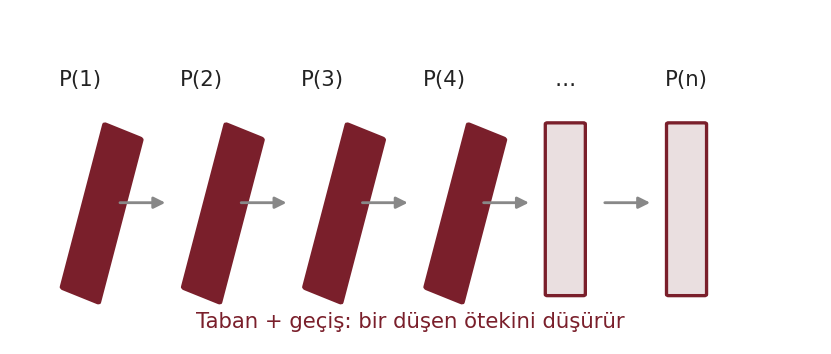
\includegraphics[width=0.85\linewidth]{figs/induction.png}
\caption{Tümevarım: taban durumu ilk taşı düşürür, geçiş adımı zinciri sürdürür.}
\end{figure}

\section{Zayıf Tümevarım Örnekleri}

\begin{tcolorbox}[bookbox,colback=cEx]\textbf{\textsf{\textcolor{cAcc}{Örnek.}}}\quad İddia: 1 + 2 + … + n = n(n+1)/2.\par\medskip{}Taban: n = 1 için sol taraf 1, sağ taraf 1·2/2 = 1. ✓\par\medskip{}Adım: P(k) doğru olsun. O hâlde 1 + … + k + (k+1) = k(k+1)/2 + (k+1) = (k+1)(k+2)/2, yani P(k+1) doğru. Böylece her n için doğrudur. ∎\end{tcolorbox}

\begin{tcolorbox}[bookbox,colback=cEx]\textbf{\textsf{\textcolor{cAcc}{Örnek.}}}\quad İddia: Her n ≥ 1 için 6 | (n³ − n).\par\medskip{}Taban: n = 1 için n³ − n = 0, 6’ya bölünür. ✓\par\medskip{}Adım: (k+1)³ − (k+1) = (k³ − k) + 3k(k+1). Birinci terim tümevarım varsayımıyla 6’ya bölünür; k(k+1) ardışık iki tam sayı olduğundan çifttir, dolayısıyla 3k(k+1) 6’ya bölünür. Toplam 6’ya bölünür. ∎\end{tcolorbox}

\section{Güçlü Tümevarım}\label{sec:guclu}

Güçlü tümevarımda, P(k+1)’i ispatlarken yalnızca P(k) değil, P(1), …, P(k)’nin tümü varsayılır. Bu, taban durumundan k+1’e kadar tüm önceki durumlara dayanmayı gerektiren ispatlarda kullanılır.

\begin{tcolorbox}[bookbox,colback=cEx]\textbf{\textsf{\textcolor{cAcc}{Örnek.}}}\quad İddia: Her n ≥ 2 doğal sayısı asalların çarpımı olarak yazılabilir.\par\medskip{}İspat (güçlü tümevarım): Taban n = 2 asaldır. n = k+1 için: ya k+1 asaldır (bitti), ya da k+1 = a·b, 2 ≤ a, b ≤ k. Tümevarım varsayımıyla a ve b asal çarpımıdır; öyleyse k+1 de asal çarpımıdır. ∎\end{tcolorbox}

\begin{tcolorbox}[bookbox,colback=cDep]\textbf{\textsf{\textcolor{cAcc}{Muhakeme/Felsefe Derinleştirmesi — Matematiksel tümevarım neden tümdengelimseldir?}}}\quad Adı yanıltıcıdır. Bölüm~\ref{chap:muhakeme-turleri}’de tümevarımsal muhakemenin sonucu yalnızca desteklediğini, garanti etmediğini görmüştük. Oysa matematiksel tümevarım, sonlu iki adımdan (taban + geçiş) hareketle sonsuz çoklukta önermenin doğruluğunu \emph{zorunlu} olarak türetir; hiçbir örneği ‘tek tek deneyip genellemez’. Bu yüzden tam anlamıyla tümdengelimsel bir çıkarımdır ve iyi sıralama ilkesine dayanır. Öğrencinin bu terim karışıklığını fark etmesi, muhakeme türleri ile ispat yöntemleri arasındaki köprüyü kurar.\end{tcolorbox}

\section{İleri Örnekler: Farklı Tümevarım Türleri}

Tümevarım yalnızca toplam formüllerinde değil; bölünebilirlik, eşitsizlik ve varlık iddialarında da çalışır. Aşağıdaki örnekler tekniğin kapsamını gösterir.

\begin{tcolorbox}[bookbox,colback=cEx]\textbf{\textsf{\textcolor{cAcc}{Örnek.}}}\quad Geometrik toplam: r ≠ 1 için 1 + r + r² + … + rⁿ = (r\textasciicircum{}(n+1) − 1)/(r − 1).\par\medskip{}Taban n = 0: sol taraf 1, sağ taraf (r − 1)/(r − 1) = 1. ✓  Adım: toplama rᵏ⁺¹ eklenirse (rᵏ⁺¹ − 1)/(r − 1) + rᵏ⁺¹ = (rᵏ⁺¹ − 1 + rᵏ⁺²  − rᵏ⁺¹)/(r − 1) = (rᵏ⁺² − 1)/(r − 1). Böylece formül n = k+1 için de doğrudur. ∎\end{tcolorbox}

\begin{tcolorbox}[bookbox,colback=cEx]\textbf{\textsf{\textcolor{cAcc}{Örnek.}}}\quad Bölünebilirlik: her n ≥ 1 için 3 | (n³ + 2n).\par\medskip{}Taban n = 1: 1 + 2 = 3, 3’e bölünür. ✓  Adım: (k+1)³ + 2(k+1) = (k³ + 2k) + 3(k² + k + 1). Birinci terim tümevarım varsayımıyla 3’e bölünür; ikinci terim açıkça 3’ün katıdır. Toplam 3’e bölünür. ∎\end{tcolorbox}

\begin{tcolorbox}[bookbox,colback=cEx]\textbf{\textsf{\textcolor{cAcc}{Örnek.}}}\quad Eşitsizlik: her n ≥ 4 için n! > 2ⁿ.\par\medskip{}Taban n = 4: 24 > 16. ✓  Adım: (k+1)! = (k+1)·k! > (k+1)·2ᵏ. k ≥ 4 olduğundan k + 1 ≥ 5 > 2, dolayısıyla (k+1)·2ᵏ > 2·2ᵏ = 2ᵏ⁺¹. Böylece (k+1)! > 2ᵏ⁺¹. ∎\end{tcolorbox}

\begin{tcolorbox}[bookbox,colback=cEx]\textbf{\textsf{\textcolor{cAcc}{Örnek.}}}\quad Güçlü tümevarımla varlık: her n ≥ 8 tam sayısı 3a + 5b (a, b ≥ 0 tam sayı) biçiminde yazılabilir.\par\medskip{}Taban: 8 = 3 + 5, 9 = 3·3, 10 = 5·2. Adım: n ≥ 11 için n − 3 ≥ 8’dir; tümevarım varsayımıyla n − 3 = 3a + 5b yazılır, buna bir 3 eklenerek n = 3(a+1) + 5b elde edilir. Üç ardışık taban durumu, adımın ‘üç geri’ gitmesini karşıladığı için gereklidir. ∎\end{tcolorbox}

\begin{tcolorbox}[bookbox,colback=cMis]\textbf{\textsf{\textcolor{cAcc}{Yaygın Kavram Yanılgıları}}}\quad \textbf{“Taban adımını atlayabilirim.” — }Taban olmadan geçiş boşta kalır; ‘tüm sayılar birbirine eşittir’ gibi saçma sonuçlar taban eksikliğinden doğar.\par\medskip{}\textbf{“Tümevarım hipotezi, ispatlamak istediğim şeyi varsaymaktır (döngüsel).” — }Hayır; P(k)’yi varsayıp P(k+1)’i türetmek döngüsel değildir. Sonsuz sayıda ‘eğer-ise’ adımını, iyi sıralama sayesinde tek seferde kurmaktır.\par\medskip{}\textbf{“Tümevarım yalnızca eşitlikler içindir.” — }Bölünebilirlik, eşitsizlik ve varlık iddiaları da tümevarımla kanıtlanır.\par\medskip{}\textbf{“Güçlü ve zayıf tümevarım farklı güçtedir.” — }İkisi mantıksal olarak denktir; ‘güçlü’ biçim yalnızca bazı ispatları kolaylaştırır.\par\medskip{}\textbf{“Adımda n = k+1’i doğrudan hesaplarım.” — }Amaç hesaplamak değil, P(k)’den P(k+1)’i türetmektir; tümevarım hipotezi mutlaka kullanılmalıdır, yoksa ispat tümevarım değildir.\end{tcolorbox}

\section{Uygulama ve Eğitime Yansıma}

Tümevarım, bilgisayar biliminin belkemiğidir: özyinelemeli (recursive) algoritmaların doğruluğu ve döngü değişmezleri (loop invariants) tümevarımla kanıtlanır. Bir öğrenci ‘taban durum + özyineleme adımı’ kalıbını tümevarımla eşleştirdiğinde, hem matematiksel ispatı hem de programlamadaki özyinelemeyi aynı fikrin iki yüzü olarak görür.

Öğretimde en sık görülen iki hata, taban adımının unutulması ve tümevarım hipotezinin hiç kullanılmamasıdır. Öğretmen, öğrenciye ‘hipotezini nerede kullandın?’ sorusunu düzenli sorarak bu boşlukları görünür kılabilir. ‘Tüm atlar aynı renktedir’ gibi klasik sahte ispatlar, hatanın tam olarak hangi adımda saklandığını tartıştırmak için güçlü bir sınıf etkinliğidir.

\section{Yüksek Lisans Derinleştirmesi: İyi Sıralama, Denklik ve Yapısal Tümevarım}

Matematiksel tümevarım ilkesi, iyi sıralama ilkesine denktir: her biri diğerinden türetilebilir. İyi sıralamadan tümevarıma geçiş şöyledir: P(n)’in doğru olmadığı sayılar kümesi S boş değilse, iyi sıralamayla S’nin bir en küçük elemanı m vardır; m > taban olduğundan m − 1 için P doğrudur, ama geçiş adımı P(m)’i verir — çelişki. Demek ki S boştur. Bu denklik, tümevarımın ‘aksiyom’ değil, doğal sayıların düzeninin bir sonucu olduğunu gösterir.

Tümevarım yalnızca sayılarla sınırlı değildir. Yapısal tümevarım (structural induction), özyinelemeli tanımlanan nesneler — ifadeler, ağaçlar, biçimsel diller — üzerinde çalışır: taban durum en basit nesnelerdir, adım ise nesneleri birleştiren kurallardır. Örneğin bir mantık formülünün her alt formülü için bir özelliğin geçerliliği yapısal tümevarımla kanıtlanır. Bu, tümevarımın ‘sıra’ değil, ‘iyi temellendirilmiş (well-founded) bir ilişki’ gerektirdiğini ortaya koyar.

Bu fikrin en genel biçimi sonlu-ötesi (transfinite) tümevarımdır: iyi sıralı herhangi bir küme üzerinde — sıra sayıları (ordinaller) dahil — tümevarım yapılabilir. Böylece ‘taban + geçiş’ şeması, sonlu doğal sayıların çok ötesine, sonsuz ama iyi sıralı yapılara taşınır. Öğretmen adayı için buradaki ders, matematiksel tümevarımın izole bir hüner değil, ‘iyi temellendirilmiş yapılarda tümdengelim’ biçimindeki derin bir ilkenin en tanıdık örneği olduğudur.

\section{Daha Fazla Uygulama: Hanoi, Küpler ve Eşitsizlik}

Tümevarımın kapsamını birkaç klasik örnekle daha genişletelim. Her biri farklı bir problem türünü — sayma, cebirsel özdeşlik, eşitsizlik — temsil eder, ama hepsi aynı taban–geçiş şemasını kullanır.

\begin{tcolorbox}[bookbox,colback=cEx]\textbf{\textsf{\textcolor{cAcc}{Örnek.}}}\quad \textbf{Hanoi Kuleleri. }n diskli Hanoi bulmacası en az 2ⁿ − 1 hamlede çözülür. Taban n = 1: tek disk 2¹ − 1 = 1 hamlede taşınır. Adım: k + 1 diski taşımak için üstteki k diski (varsayımla 2ᵏ − 1 hamle), en alttaki diski (1 hamle) ve k diski tekrar (2ᵏ − 1 hamle) taşırız; toplam 2(2ᵏ − 1) + 1 = 2ᵏ⁺¹ − 1. Bulmacanın özyinelemeli yapısı, tümevarımın doğal habitatıdır. ∎\end{tcolorbox}

\begin{tcolorbox}[bookbox,colback=cEx]\textbf{\textsf{\textcolor{cAcc}{Örnek.}}}\quad \textbf{Küplerin toplamı. }1³ + 2³ + … + n³ = (n(n + 1)/2)². Taban n = 1: 1 = 1². Adım: tümevarım varsayımına (k + 1)³ eklenip düzenlenince ((k + 1)(k + 2)/2)² elde edilir. Şaşırtıcı olan, ilk n küpün toplamının, ilk n sayının toplamının karesi olmasıdır — sayma ve cebir arasında zarif bir köprü. ∎\end{tcolorbox}

\begin{tcolorbox}[bookbox,colback=cEx]\textbf{\textsf{\textcolor{cAcc}{Örnek.}}}\quad \textbf{Bernoulli eşitsizliği. }x ≥ −1 ve n ≥ 0 için (1 + x)ⁿ ≥ 1 + nx. Taban n = 0: 1 ≥ 1. Adım: (1 + x)ᵏ⁺¹ = (1 + x)(1 + x)ᵏ ≥ (1 + x)(1 + kx) = 1 + (k + 1)x + kx² ≥ 1 + (k + 1)x, çünkü kx² ≥ 0. Bu eşitsizlik analizde, limit ve yakınsaklık hesaplarında sürekli kullanılır. ∎\end{tcolorbox}

\section{Özyineleme ve Algoritma Doğruluğu}

Tümevarımın belki en yaygın çağdaş uygulaması bilgisayar bilimindedir. Özyinelemeli (recursive) bir fonksiyon, taban durum ile ‘kendini daha küçük girdide çağırma’ adımından oluşur — tam olarak tümevarımın taban ve geçiş adımlarına karşılık gelir. Bir özyinelemeli algoritmanın doğruluğu, çıktısının doğru olduğu iddiasının tümevarımla kanıtlanmasıyla kurulur; sonlanması ise girdinin her çağrıda ‘iyi temellendirilmiş’ biçimde küçülmesiyle güvence altına alınır.

Aynı fikir döngüler için ‘döngü değişmezi’ (loop invariant) olarak karşımıza çıkar: döngünün her yinelemesinde korunan bir özellik, taban (döngüden önce) ve geçiş (her yineleme) adımlarıyla kanıtlanır; döngü bittiğinde bu değişmez, istenen sonucu verir. Böylece bir öğrenci ‘taban + adım’ kalıbını öğrendiğinde, hem matematiksel bir teoremi kanıtlayabilir hem de bir programın neden doğru çalıştığını gerekçelendirebilir. Tümevarım, bu yönüyle matematik ile hesaplama arasındaki en somut bağlardan biridir ve öğretmen adayına konunun ‘yalnızca formül kanıtlamak’ olmadığını gösterir.

\section{İki Uzun Örnek: Bölünebilirlik ve Karo Döşeme}

Tümevarımın çok yönlülüğünü, biri klasik biri görsel iki örnekle daha pekiştirelim. Bu örnekler, tekniğin cebirden geometriye uzanan kapsamını gösterir.

\begin{tcolorbox}[bookbox,colback=cEx]\textbf{\textsf{\textcolor{cAcc}{Örnek.}}}\quad Bölünebilirlik: her n ≥ 1 için 7 | (8ⁿ − 1).\par\medskip{}Taban n = 1: 8 − 1 = 7, 7’ye bölünür. ✓  Adım: 8ᵏ⁺¹ − 1 = 8·8ᵏ − 1 = 8(8ᵏ − 1) + 7. İlk terim tümevarım varsayımıyla 7’ye bölünür, ikinci terim 7’dir; toplam 7’ye bölünür. ∎  (Aynı sonuç 8 ≡ 1 (mod 7) kongrüansıyla da anında görülür — Bölüm~\ref{chap:kongruanslar}; iki yöntem birbirini aydınlatır.)\end{tcolorbox}

\begin{tcolorbox}[bookbox,colback=cEx]\textbf{\textsf{\textcolor{cAcc}{Örnek.}}}\quad Teleskopik toplam: 1/(1·2) + 1/(2·3) + … + 1/(n(n+1)) = n/(n+1).\par\medskip{}Taban n = 1: 1/(1·2) = 1/2 = 1/2. ✓  Adım: n/(n+1) + 1/((n+1)(n+2)) toplamını paydada birleştirirsek (n(n+2) + 1)/((n+1)(n+2)) = (n+1)²/((n+1)(n+2)) = (n+1)/(n+2). Böylece formül n+1 için de doğrudur. Bu tür toplamlar, her terimin ‘bir öncekini götürdüğü’ teleskopik yapıyı sergiler. ∎\end{tcolorbox}

Şimdi görsel bir örnek: bir 2ⁿ × 2ⁿ satranç tahtasından herhangi bir kare çıkarılırsa, kalan bölge L biçimli üçlü karolarla (her biri üç kareyi kaplayan ‘L-tromino’) tam olarak döşenebilir.

\begin{tcolorbox}[bookbox,colback=cEx]\textbf{\textsf{\textcolor{cAcc}{Örnek.}}}\quad L-tromino döşemesi (güçlü/olağan tümevarım).\par\medskip{}Taban n = 1: 2 × 2 tahtadan bir kare çıkınca geriye tam olarak bir L-tromino biçimi kalır. ✓  Adım: 2ᵏ⁺¹ × 2ᵏ⁺¹ tahtayı dört adet 2ᵏ × 2ᵏ çeyreğe böleriz. Çıkarılan kare bir çeyrektedir; o çeyrek tümevarım varsayımıyla döşenir. Kalan üç çeyreğin merkeze bakan köşelerine bir L-tromino yerleştirerek her birinde ‘çıkarılmış bir kare’ etkisi yaratırız; böylece o üç çeyrek de varsayımla döşenir. ∎  Bu ispat, tümevarımın geometrik bir yapıyı nasıl parçalayıp özyinelemeli biçimde çözdüğünü gösterir.\end{tcolorbox}

Bu üç örnek — cebirsel bölünebilirlik, teleskopik toplam ve geometrik döşeme — tümevarımın tek bir formül türüne bağlı olmadığını gösterir. Ortak olan, problemi ‘bir küçüğüne’ indirgeyip varsayımı kullanmaktır. Öğretmen adayı için buradaki mesaj, tümevarımın ezberlenecek bir kalıp değil, çok farklı bağlamlarda yeniden keşfedilebilecek bir düşünme aracı olduğudur; bu esneklik, öğrencinin yöntemi anlamlı biçimde sahiplenmesinin ön koşuludur.

\begin{tcolorbox}[bookbox,colback=cDef]\textbf{\textsf{\textcolor{cAcc}{Tarihsel Not}}}\quad Matematiksel tümevarımın açık ilk kullanımı çoğu zaman Blaise Pascal’a (1654, Traité du triangle arithmétique) atfedilir; ancak yöntemin izleri Öklid’e, Hintli matematikçilere ve on altıncı yüzyılda Francesco Maurolico’ya kadar uzanır. ‘Tümevarım’ (induction) terimini bu bağlamda İngilizce’ye yerleştiren John Wallis ve Augustus De Morgan oldu. On dokuzuncu yüzyılda Giuseppe Peano ise tümevarımı doğal sayıların tanımlayıcı aksiyomlarından biri hâline getirerek, onu bir ‘hüner’ olmaktan çıkarıp ℕ’nin özünün parçası yaptı.\end{tcolorbox}

\section{Görsel Düşünme ve Hatalı Tümevarımlar}

Tümevarım ilkesini bir kez anlamak kolaydır; onu doğru \emph{kullanmak} ise dikkat ister. Bu kısımda önce zayıf ve güçlü tümevarımın mantıksal yapısını bir şemayla karşılaştırıyor, ardından bir eşitsizlik ailesinin grafiğini inceliyor ve son olarak öğrencilerin en sık düştüğü üç tuzağı çözümlü örneklerle ele alıyoruz.

\begin{figure}[htbp]
\centering
\resizebox{\linewidth}{!}{%
\begin{tikzpicture}[x=1.55cm,y=1cm,p/.style={circle,draw=acc,fill=accl,line width=.8pt,minimum size=9mm,font=\sffamily\small}]
\node[font=\sffamily\small\bfseries,anchor=west] at (-.4,1.15) {Zayıf tümevarım: $P(k)\Rightarrow P(k+1)$};
\foreach \i in {1,...,6}{\node[p] (a\i) at (\i,0) {$P(\i)$};}
\foreach \i [evaluate=\i as \j using int(\i+1)] in {1,...,5}{\draw[arr] (a\i)--(a\j);}
\node[font=\sffamily\small] at (6.8,0) {$\cdots$};
\node[font=\sffamily\small\bfseries,anchor=west] at (-.4,-1.45) {Güçlü tümevarım: $P(1)\wedge\cdots\wedge P(k)\Rightarrow P(k+1)$};
\foreach \i in {1,...,6}{\node[p,draw=grn,fill=grnl] (b\i) at (\i,-2.6) {$P(\i)$};}
\foreach \i in {1,...,5}{\foreach \j in {\i,...,5}{\pgfmathtruncatemacro{\t}{\j+1}
  \ifnum\j=\i \draw[arr,grn] (b\i)--(b\t); \else \draw[arr,grn!70,line width=.5pt] (b\i.south) to[bend right=28] (b\t.south);\fi}}
\node[font=\sffamily\small] at (6.8,-2.6) {$\cdots$};
\node[small lbl,anchor=west,text width=3.2cm] at (7.2,-.2) {Her halka yalnızca bir öncekine dayanır.};
\node[small lbl,anchor=west,text width=3.2cm] at (7.2,-2.8) {Her halka, kendisinden önceki \emph{bütün} halkalara dayanabilir.};
\end{tikzpicture}}%
\caption{Zayıf ve güçlü tümevarımın gerekçelendirme yapısı. Güçlü tümevarım daha fazla varsayım kullanır; ama iki ilke doğal sayılarda birbirine denktir.}
\end{figure}

\begin{ornek}[\textbf{Küplerin toplamı bir karedir.}]
Her $n\ge1$ için
\[
1^3+2^3+\cdots+n^3=\Bigl(\frac{n(n+1)}{2}\Bigr)^2 .
\]
\emph{Taban:} $n=1$ için iki taraf da 1’dir. \emph{Adım:} Eşitlik $n=k$ için doğru olsun. O hâlde
\begin{align*}
\sum_{i=1}^{k+1}i^3&=\frac{k^2(k+1)^2}{4}+(k+1)^3\\
&=\frac{(k+1)^2\bigl(k^2+4k+4\bigr)}{4}=\Bigl(\frac{(k+1)(k+2)}{2}\Bigr)^2 .
\end{align*}
Böylece eşitlik $n=k+1$ için de doğrudur. Sonuç şaşırtıcı bir özdeşlik verir: $1^3+\cdots+n^3=(1+\cdots+n)^2$. Sonucun \emph{keşfi} büyük olasılıkla ilk birkaç değerin ($1,9,36,100$) tam kare olduğunun fark edilmesiyle başlar (tümevarımsal gözlem); \emph{gerekçesi} ise yukarıdaki tümdengelimsel adımdır.
\end{ornek}

\begin{ornek}[\textbf{Bernoulli eşitsizliği: varsayım nerede kullanılıyor?}]
$x\ge-1$ ve $n\ge1$ için $(1+x)^n\ge1+nx$ olduğunu gösterelim. Taban $n=1$ için eşitliktir. $(1+x)^k\ge1+kx$ olsun. Her iki tarafı $1+x$ ile çarpalım:
\[
(1+x)^{k+1}\ \ge\ (1+kx)(1+x)=1+(k+1)x+kx^2\ \ge\ 1+(k+1)x .
\]
İlk eşitsizlikte bir eşitsizliği \emph{negatif olmayan} bir sayıyla çarptık; $x\ge-1$ koşulu tam olarak burada kullanılır. İkinci eşitsizlik $kx^2\ge0$ olgusudur. Koşulu kaldırırsak sonuç bozulabilir: $x=-4$, $n=3$ için $(1+x)^3=-27$ iken $1+3x=-11$ olur ve $-27\ge-11$ yanlıştır. Bir tümevarım ispatında \emph{her varsayımın hangi satırda kullanıldığını} işaretlemek, ispatı anlamanın en kısa yoludur.
\end{ornek}

\begin{figure}[htbp]
\centering
\begin{tikzpicture}
\begin{axis}[width=.82\linewidth,height=5cm,ybar,bar width=6pt,xlabel={$n$},ylabel={değer},xtick={1,...,8},ymin=0,ymax=270,
  axis lines*=left,tick label style={font=\sffamily\scriptsize},label style={font=\sffamily\small},
  legend style={at={(0.03,0.97)},anchor=north west,font=\sffamily\scriptsize,draw=none,fill=none}]
\addplot[fill=acc!70,draw=acc] coordinates {(1,2)(2,4)(3,8)(4,16)(5,32)(6,64)(7,128)(8,256)};
\addplot[fill=warm!60,draw=warm] coordinates {(1,1)(2,4)(3,9)(4,16)(5,25)(6,36)(7,49)(8,64)};
\legend{$2^n$,$n^2$}
\end{axis}
\end{tikzpicture}
\caption{$2^n$ ile $n^2$: $n=3$’te $n^2$ öndedir, $n=2$ ve $n=4$’te eşittirler, $n\ge5$ için $2^n$ kesin olarak büyüktür. ‘Her $n$ için $2^n>n^2$’ yanlış; ‘her $n\ge5$ için’ doğrudur. Taban durumunun seçimi, iddianın kendisinin bir parçasıdır.}
\end{figure}

\subsection{Üç Tipik Hata}

\begin{yanilgi}[Hata 1 — Taban adımını atlamak]
‘$n^2+n+1$ her $n$ için çifttir’ iddiasını düşünelim. Adım kusursuz görünür: $k^2+k+1$ çiftse
\[
(k+1)^2+(k+1)+1=(k^2+k+1)+2(k+1)
\]
de çifttir. Oysa iddia \emph{her} $n$ için yanlıştır: $n^2+n=n(n+1)$ çift olduğundan $n^2+n+1$ daima tektir. Adım ‘boşluğa’ kurulmuş bir köprüdür; hiçbir taş ilk kez düşmemiştir.
\end{yanilgi}

\begin{yanilgi}[Hata 2 — Kanıtlanacak olanı adımda varsaymak]
Bazı öğrenciler adımı şöyle yazar: ‘$P(k+1)$ doğru olsun; o hâlde … öyleyse $P(k)$ doğrudur.’ Bu, gerekirliğin yönünü ters çevirir. Adımda varsayılan $P(k)$’dır; ulaşılması gereken $P(k+1)$’dir. Eşitlik ispatlarında güvenli yol, $P(k+1)$’in sol tarafından başlayıp $P(k)$’yı \emph{kullanarak} sağ tarafa varmaktır.
\end{yanilgi}

\begin{yanilgi}[Hata 3 — Adımın küçük değerlerde çalışmaması]
‘Bütün atlar aynı renktir’ yanıltmacasında (Alıştırma 5’teki ‘herkes aynı yaştadır’ sahte ispatı da aynı yapıdadır) adım, ‘ilk $k$ at’ ile ‘son $k$ at’ gruplarının ortak bir ata sahip olmasına dayanır. Bu, $k\ge2$ için doğrudur ama $k=1$’den $k+1=2$’ye geçişte ortak at yoktur. Adımın \emph{bütün} $k\ge n_0$ değerlerinde geçerli olduğunu denetlemek gerekir; en küçük $k$ değeri çoğu zaman en tehlikeli olanıdır.
\end{yanilgi}

\begin{sinif}[Sınıfta · Tümevarım ispat şablonu]
Aşağıdaki şablonu öğrencilere boş olarak verin ve her ispatta doldurtun. Şablon, ispatın mantıksal iskeletini görünür kılar; özellikle ‘Hipotez nerede kullanıldı?’ satırı, öğrencinin hipotezi gerçekten kullanıp kullanmadığını denetler.
\begin{center}\small
\renewcommand{\arraystretch}{1.25}
\begin{tabularx}{.95\linewidth}{>{\bfseries\raggedright\arraybackslash}p{2.6cm}X}
\toprule
Önerme $P(n)$ & $1+3+\cdots+(2n-1)=n^2$, $n\ge1$\\
Taban & $n=1$: $1=1^2$ \checkmark\\
Hipotez & $1+3+\cdots+(2k-1)=k^2$ olsun.\\
Hedef & $1+3+\cdots+(2k+1)=(k+1)^2$\\
Hipotez nerede kullanıldı? & İlk $k$ terimin toplamı yerine $k^2$ yazıldı.\\
Sonuç & Tümevarım ilkesiyle $P(n)$ her $n\ge1$ için doğrudur.\\
\bottomrule
\end{tabularx}
\end{center}
\end{sinif}

\section*{Alıştırmalar}

\reviewitem{1}{Her n ≥ 1 için 1·2 + 2·3 + … + n(n + 1) = n(n + 1)(n + 2)/3 olduğunu tümevarımla gösterin.}

\reviewitem{2}{Her n ≥ 5 için 2ⁿ > n² olduğunu tümevarımla gösterin (taban durumunu dikkatle seçin).}

\reviewitem{3}{Düzlemdeki n doğru, düzlemi en fazla kaç bölgeye ayırır? Bir formül tahmin edip tümevarımla kanıtlayın.}

\reviewitem{4}{Fibonacci dizisi için Fₙ < 2ⁿ olduğunu güçlü tümevarımla gösterin.}

\reviewitem{5}{“n kişilik her grupta herkes aynı yaştadır” sahte ispatını yazın ve hatanın tam olarak hangi adımda gizlendiğini belirtin.}

\section*{Bölüm Özeti}

\begin{itemize}\setlength{\itemsep}{2pt}\setlength{\parskip}{0pt}
\item Tümevarım taban ve geçiş adımlarından oluşur; güçlü biçimi önceki tüm durumları varsayar.
\item Yöntem, iyi sıralama ilkesine dayanır ve sonsuz önermeyi sonlu adımla türetir.
\item Adına rağmen matematiksel tümevarım tümdengelimsel bir yöntemdir.
\end{itemize}

\section*{Gözden Geçirme Soruları}

\reviewitem{1}{‘Tüm atlar aynı renktir’ sözde ispatındaki hata tümevarımın hangi adımındadır?}

\reviewitem{2}{1 + 3 + 5 + … + (2n−1) = n² eşitliğini tümevarımla ispatlayınız.}

\reviewitem{3}{Neden bazı ispatlarda zayıf tümevarım yetmez de güçlü tümevarım gerekir?}

\section*{Çoktan Seçmeli Sorular}

\mcqq{1}{Tümevarımın hangi adımı ‘P(k) ⇒ P(k+1)’ biçimindedir?}

\mcqo{A}{Taban}

\mcqo{B}{Geçiş (adım)}

\mcqo{C}{Sonuç}

\mcqo{D}{Olumsuzlama}

\mcqa{B}{Geçiş adımı P(k)’den P(k+1)’e götürür.}

\mcqq{2}{Matematiksel tümevarım hangi ilkeye dayanır?}

\mcqo{A}{Seçim aksiyomu}

\mcqo{B}{İyi sıralama ilkesi}

\mcqo{C}{De Morgan}

\mcqo{D}{Modus tollens}

\mcqa{B}{Tümevarım iyi sıralama ilkesine dayanır.}

\mcqq{3}{Muhakeme türü olarak matematiksel tümevarım nedir?}

\mcqo{A}{Tümevarımsal}

\mcqo{B}{Abdüktif}

\mcqo{C}{Tümdengelimsel}

\mcqo{D}{Analojik}

\mcqa{C}{Sonlu adımdan sonsuz sonuç zorunlu türetildiği için tümdengelimseldir.}

\mcqq{4}{Önceki tüm durumları varsayan biçim hangisidir?}

\mcqo{A}{Zayıf tümevarım}

\mcqo{B}{Güçlü tümevarım}

\mcqo{C}{Kontrapozitif}

\mcqo{D}{Doğrudan ispat}

\mcqa{B}{Güçlü tümevarım P(1)…P(k)’nin tümünü varsayar.}

\mcqq{5}{Taban adımı neyi gösterir?}

\mcqo{A}{Genel adımı}

\mcqo{B}{İlk durumun (n = 1) doğruluğunu}

\mcqo{C}{Sonucu}

\mcqo{D}{Olumsuzunu}

\mcqa{B}{Taban, ilk durumun (n=1) doğruluğunu kurar.}

\mcqq{6}{1 + 2 + … + n toplamı neye eşittir?}

\mcqo{A}{n²}

\mcqo{B}{n(n−1)/2}

\mcqo{C}{n(n+1)/2}

\mcqo{D}{2n}

\mcqa{C}{Aritmetik dizi toplamı n(n+1)/2’dir.}

\mcqq{7}{İlk n tek sayının toplamı 1 + 3 + … + (2n−1) neye eşittir?}

\mcqo{A}{n(n+1)/2}

\mcqo{B}{n²}

\mcqo{C}{2n − 1}

\mcqo{D}{n(n+1)}

\mcqa{B}{İlk n tek sayının toplamı n²’dir.}

\mcqq{8}{“Tüm atlar aynı renktir” sözde ispatındaki hata nerededir?}

\mcqo{A}{Taban yanlıştır}

\mcqo{B}{Geçiş adımındaki örtüşme küçük n’de geçersizdir}

\mcqo{C}{Sonuç doğrudur}

\mcqo{D}{İlke yanlıştır}

\mcqa{B}{Örtüşme küçük n’de sağlanmaz; hata geçiş adımındadır.}

\mcqq{9}{6 | (n³ − n) ispatında geçiş adımında 3k(k+1) neden 6’ya bölünür?}

\mcqo{A}{k daima çifttir}

\mcqo{B}{k(k+1) ardışık olduğundan çifttir, 3·çift = 6’nın katı}

\mcqo{C}{3 tek olduğundan}

\mcqo{D}{Bölünmez}

\mcqa{B}{k(k+1) ardışık olduğundan çifttir; 3·çift, 6’ya bölünür.}

\mcqq{10}{“Her n ≥ 2 asalların çarpımıdır” güçlü tümevarımında taban nedir?}

\mcqo{A}{n = 2 asaldır}

\mcqo{B}{n = 1}

\mcqo{C}{n = 0}

\mcqo{D}{Taban gerekmez}

\mcqa{A}{Taban n=2’dir ve 2 asaldır.}

\mcqq{11}{Tümevarım sonsuz çoklukta önermeyi nasıl kanıtlar?}

\mcqo{A}{Hepsini tek tek deneyerek}

\mcqo{B}{Sonlu iki adımla zorunlu türeterek}

\mcqo{C}{Olasılıkla}

\mcqo{D}{Örneklerle}

\mcqa{B}{İki sonlu adım (taban+geçiş) sonsuz önermeyi zorunlu kılar.}

\mcqq{12}{İyi sıralama ilkesi ne der?}

\mcqo{A}{Her küme sıralıdır}

\mcqo{B}{Boştan farklı her ℕ alt kümesinin en küçük elemanı vardır}

\mcqo{C}{ℝ iyi sıralıdır}

\mcqo{D}{Her küme sonludur}

\mcqa{B}{İyi sıralama: ℕ’nin boştan farklı her alt kümesinin en küçüğü vardır.}

\mcqq{13}{Zayıf tümevarımda geçiş adımında ne varsayılır?}

\mcqo{A}{P(1)…P(k) hepsi}

\mcqo{B}{Yalnızca P(k)}

\mcqo{C}{P(k+1)}

\mcqo{D}{Hiçbiri}

\mcqa{B}{Zayıf biçim yalnızca bir önceki durumu (P(k)) varsayar.}

\mcqq{14}{Geçiş adımı ispatlanmazsa ne olur?}

\mcqo{A}{Taban yeterlidir}

\mcqo{B}{İlke değişir}

\mcqo{C}{Sonuç garanti edilmez}

\mcqo{D}{Yine doğrudur}

\mcqa{C}{Geçiş kanıtlanmazsa zincir kırılır, sonuç garanti edilmez.}

\mcqq{15}{2ⁿ > n (n ≥ 1) ifadesi tipik olarak hangi yöntemle kanıtlanır?}

\mcqo{A}{Kontrapozitif}

\mcqo{B}{Tümevarım}

\mcqo{C}{Doğruluk tablosu}

\mcqo{D}{Sayma}

\mcqa{B}{Eşitsizlik n üzerinden tümevarımla kanıtlanır.}

\mcqq{16}{Klasik biçimiyle matematiksel tümevarım hangi sayılarda çalışır?}

\mcqo{A}{Gerçel sayılar}

\mcqo{B}{Doğal sayılar}

\mcqo{C}{Karmaşık sayılar}

\mcqo{D}{İrrasyoneller}

\mcqa{B}{Klasik tümevarım doğal sayılar üzerinde işler.}

\mcqq{17}{Geçiş adımında varsayılan P(k) önermesine ne ad verilir?}

\mcqo{A}{Sonuç}

\mcqo{B}{Tümevarım hipotezi}

\mcqo{C}{Taban}

\mcqo{D}{Aksiyom}

\mcqa{B}{Varsayılan P(k)’ye tümevarım hipotezi denir.}

\mcqq{18}{Bir tümevarım ispatı en az kaç adım içerir?}

\mcqo{A}{Bir}

\mcqo{B}{İki (taban ve geçiş)}

\mcqo{C}{Üç}

\mcqo{D}{Sonsuz}

\mcqa{B}{En az iki adım gerekir: taban ve geçiş.}

\mcqq{19}{Güçlü tümevarım ne zaman gerekir?}

\mcqo{A}{Her zaman}

\mcqo{B}{P(k+1) önceki birden çok duruma bağlıysa}

\mcqo{C}{Hiçbir zaman}

\mcqo{D}{Taban yoksa}

\mcqa{B}{Sonuç önceki birçok duruma bağlıysa güçlü biçim gerekir.}

\mcqq{20}{“Matematiksel tümevarım” adı neden yanıltıcıdır?}

\mcqo{A}{Aslında tümevarımsaldır}

\mcqo{B}{Tümdengelimsel olduğu hâlde ‘tümevarım’ denir}

\mcqo{C}{Abdüktiftir}

\mcqo{D}{Analojiktir}

\mcqa{B}{Yöntem tümdengelimseldir; ‘tümevarım’ adı tarihsel bir yanıltmadır.}


\clearpage

\clearpage